\documentclass{article}

\usepackage{graphicx}
\usepackage{hyperref}
\usepackage{amsmath}
\usepackage{amssymb}
\usepackage{blkarray}
\usepackage{cancel}
\usepackage{fancyhdr}
\usepackage{enumitem}
\usepackage{lscape}
\usepackage{listings}
\usepackage{color}
\usepackage{pdfpages}
\usepackage{yfonts}
\usepackage{caption}
\usepackage{natbib}
\definecolor{dkgreen}{rgb}{0,0.6,0}
\definecolor{gray}{rgb}{0.5,0.5,0.5}
\definecolor{mauve}{rgb}{0.58,0,0.82}

\usepackage{xcolor}

\lstdefinestyle{base}{
  inputencoding=latin10,
  emptylines=1,
  breaklines=true,
  basicstyle=\small\ttfamily,
  moredelim=**[is][\color{red}]{@}{@},
}

\newcommand{\norm}[1]{\left\lVert#1\right\rVert}

%% Define a HUGE 
\makeatletter
\newcommand\HUGE{\@setfontsize\Huge{50}{60}}
\makeatother

\hypersetup{
    colorlinks=true,
    linkcolor=blue,
    filecolor=magenta,      
    urlcolor=cyan    
}

\begin{document}             % End of preamble and beginning of text.

 
%titlepage
\thispagestyle{empty}
\begin{center}
\begin{minipage}{.9\linewidth}
\flushright
	      		 

\includegraphics[width=0.5\linewidth]{univie.jpg}\par
\vspace{1.5cm}
\centering 	
    % Title
	{\scshape{\HUGE A4 Report \par}}
	\vspace{1cm}
	%Thesis title
    {\scshape{\Large Course: VIS WS '18 \qquad  date: 13.12.2018\par}}
	\vspace{1cm}

 {\Large Name : Robert Ernstbrunner \\ Matnr.: 01403753 \hspace{2.2cm} \ \par}
 	\vspace{.7cm}

 

\end{minipage}
\end{center}
\clearpage

\section{Introduction}

The ornithology student \textit{Mitch Vogel} (yes, he's a birdwatcher named \textit{Vogel}) needs our help in visualizing his data in order to advance in his investigations. There is an observed decline in the nesting \textit{Rose-crested Blue Pipit} in the \textit{Boonsong Lekagul Nature Preserve} and Mitch thinks the traffic going through the preserve might have to do with it.
He reckons that traffic noise might overshadow mating calls or that invading campers might scare away the birds from their habitat areas. \\
The data was collected by park rangers who work as caretakers of the nature preserve. They gave Mitch additional explanations about the data together with a map. 

\section{Data, Users, Tasks}
The park rangers monitor the traffic through the preserve with the help of sensors. Tickets are assigned to vehicles at the entry gates that get scanned by these sensors when the vehicles pass by them.
\begin{itemize}

\item In summary there are seven different vehicle categories:

	\begin{enumerate}
	\item \textit{Cars} and \textit{motorcycles} count as one type.
	\item There are three types of \textit{trucks} (differentiated by their number of axles).
	\item There are two types of \textit{buses}.
	\item The seventh type consists of \textit{park service trucks} that are used by the rangers who have access to all areas.
	\end{enumerate}

\item There are five different sensor types:

	\begin{enumerate}
	\item Vehicles that enter or leave the preserve are tracked at \textit{entrance gates}.
	\item \textit{General gates} act as control points to monitor the traffic flow.
	\item Special gates, which are simply referred to as \textit{gates}, prevent general traffic from entering restricted paths. These gates can only be opened by rangers.
	\item \textit{Ranger-stops} represent the working areas for rangers. Some are cut off from general traffic and some aren't. That's why some of their sensors also collect general traffic information while others don't.
	\item Finally \textit{camping} sensors monitor visitors, that enter or exit a camping ground.
	\end{enumerate}
\newpage
\item Additional information about the dataset:

	\begin{enumerate}		
	\item Traffic either passes through the preserve, stays as day campers or stays as extended campers.
	\item Rangers reside at the southeast ranger-stop when they are not working.
	\item The speed limit is 25 mph.
	\item Summertime is not included in the sensor measurements.
	\item Traffic going southward from entrance gates \textit{three} and \textit{four} are not represented on the map and are not tracked.
	\end{enumerate}

\item Data snippet:\\
	\noindent\rule{9.3cm}{1pt}\\
	\texttt{Timestamp,car-id,car-type,gate-name}\\
	\texttt{2015-05-01 00:15:13,20151501121513-39,2,entrance4}\\
	\texttt{2015-05-01 00:32:47,20151501121513-39,2,entrance2}\\
	\texttt{2015-05-01 01:12:42,20151201011242-330,5,entrance0}\\
	\noindent\rule{9.3cm}{1pt}\\

	The data set consists of the following parameters:

	\begin{enumerate}
	\item \textit{Timestamp} \textcolor{red}{(quantitative)} contains the date and time the sensor was triggered.
	\item Entering vehicles are assigned with a \textit{car-ID} \textcolor{olive}{(nominal)} at the \textit{entry gates}.
	\item The \textit{Car-type} \textcolor{olive}{(nominal)} specifies a vehicle according to their type and number of axles. A park vehicle gets additionally marked with a \textit{'P'}.
	\item The \textit{Gate-name} \textcolor{olive}{(nominal)} is the name of the sensors themselves. The same names can also be found on the map.
	\end{enumerate}

\item The preserve:\\
	The \textit{preserve} is open to the public 24 hours a day all year long. It is visited by naturalists of all ages, photographers and explorers. It is used for hiking, camping, nature study, \textit{birdwatching}, photography and cycling. The preserve can be entered through five entrances by paying an access fee. According to the map, it comprises nine camping areas.

\item The included map is presented in \texttt{\hyperref[fig:map]{Figure~\ref{fig:map}}}.
The map consists of a black background with white roads and type-colored gate labels. It may be used as a template by the flow map visualization (\hyperref[fig:design2]{design 2}).

	\begin{figure}
		\centering
		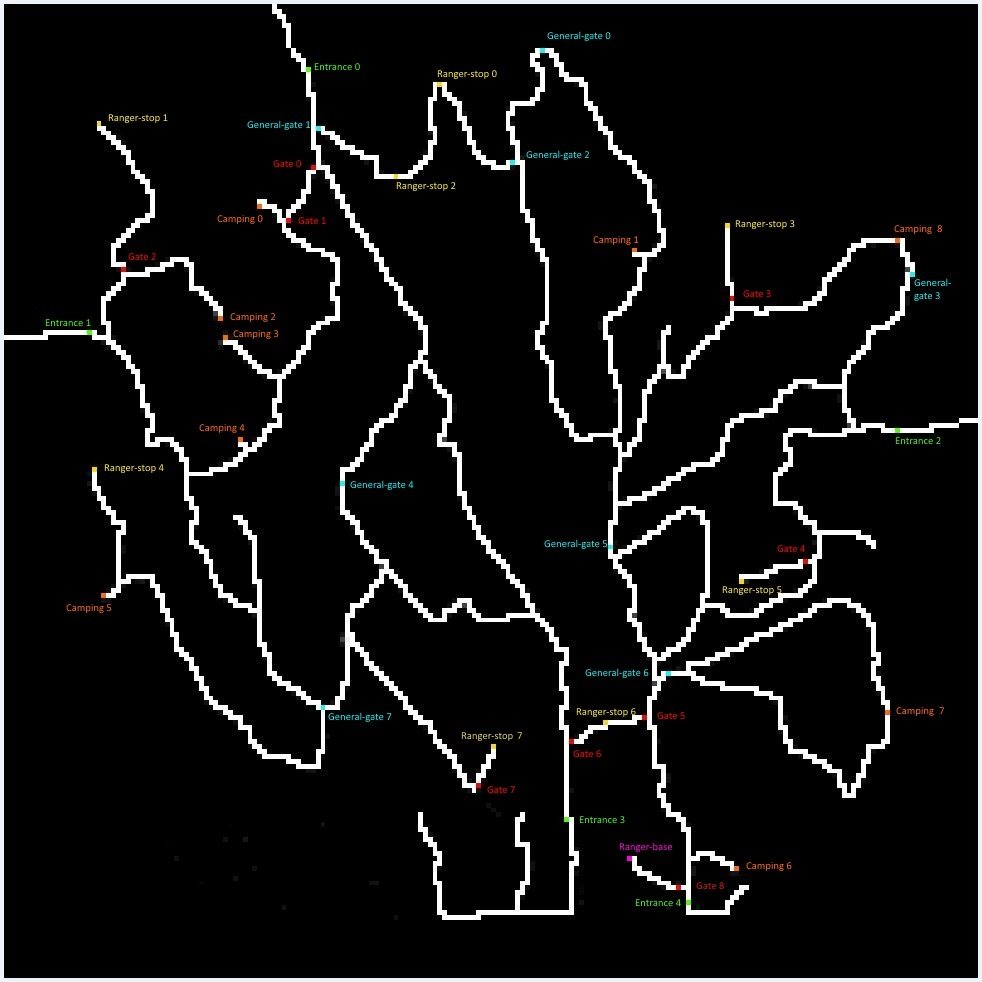
\includegraphics[scale=0.4]{Lekagul_Roadways_labeled_v2.jpg}
		\caption{the rangers map}
		\label{fig:map}
	\end{figure}	

\end{itemize}

\section{Designs}
\subsection*{Design 1} 

\begin{figure}
	\centering
	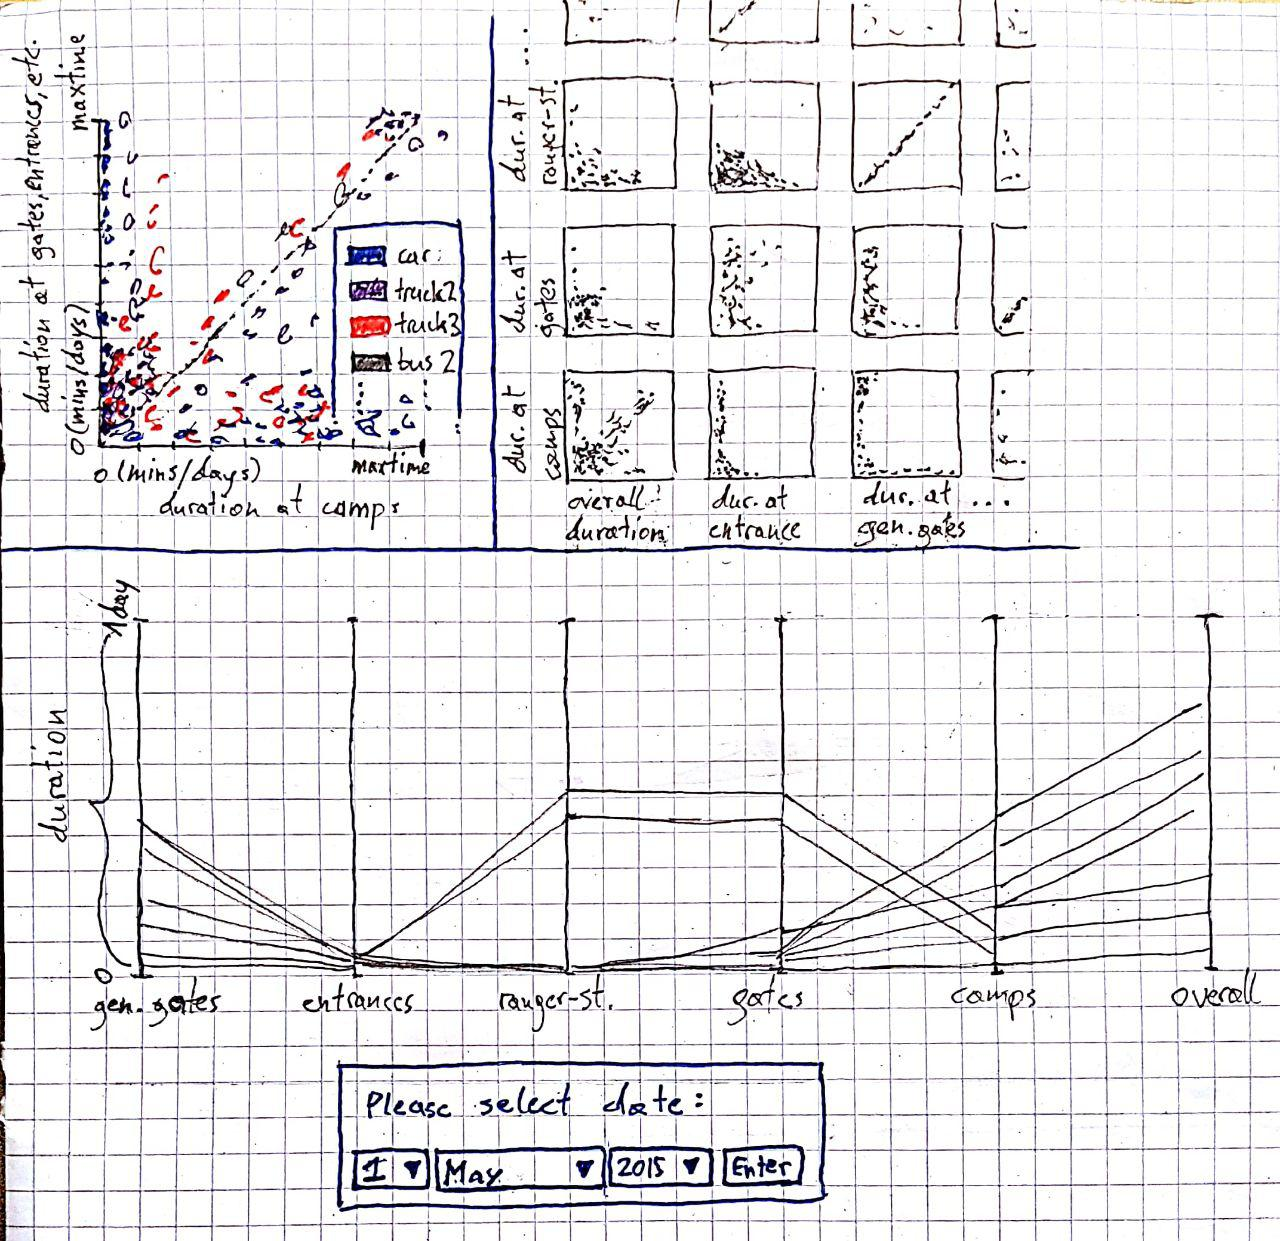
\includegraphics[scale=.45]{Design1.jpg}
	\caption{Design 1}
	\label{fig:design1}
\end{figure}

\paragraph{Visualizing behavior inside the preserve.}
For my first design (\texttt{\hyperref[fig:design1]{Figure~\ref{fig:design1}}}) I concluded that \textit{Mitch} might wants to gain insight on the traffic behavior inside the preserve. Therefore, I tried to find possible correlations between the time spent at different sensors over a single day. The most significant separator between sensor types would be the one between camp sensors and the rest. Having a closer look at relations between these two sensor types might answer the question if most of the visitors are serious (longterm) campers or just visitors/explorers spending their time mostly elsewhere. This might answer \textit{Mitchs} question if campers are mainly responsible for the decline in birds. Therefore, I drew a scatterplot in the left upper corner. The horizontal axis shows the duration spent at camps and the vertical axis shows the duration spent elsewhere. The dots represent the vehicles and since there are only seven categories, I decided to distinguish them by color.\\
Just examining the relation between camp sensors and the rest might lead to fast conclusions but it might not be enough to gain deeper insight and understanding of the data. Therefore, I sketched a scatterplot matrix (\textit{SPLOM}) right next to the scatterplot to reveal more details about the time spent at each sensor type and their correlation to one another. I also included the overall duration to (hopefully) make it even more insightful (it might be a good idea to limit the overall duration for a vehicle to a single day in order to preserve good visibility). The \textit{SPLOM} requires a table with ordinal data as input. Therefore, a table with duration at different sensor types has to be computed from the data. I was thinking about eventually removing the redundant upper triangle together with the diagonal, in order to save space (this is commonly done \citep{munzner2015visualization}), but then I realized that this might inhibit readability for \textit{Mitch} who might have never seen a \textit{SPLOM} before. I think someone in the \textit{VIS} course once said \textit{having to explain a visualization is mostly a sign for a bad visualization}. Also, I was thinking that the \textit{data ink ratio} is not affected as long as the (redundant and transposed) data in the upper triangle is justified. It could be argued that \textit{Mitch} might not understand the \textit{SPLOM} either way. That's one of the disatvantages of \textit{SPLOMS}. They might eventually reveal deeper information but are initially harder to read and understand.\\
Parallel coordinates (\textit{PC}), on the other hand, are more accessible, at least to me. That's why I also included them in the design below the scatterplot and \textit{SPLOM}. \textit{PC}, like the \textit{SPLOM}, also show correlations, but through different kinds of visual patterns. While a dot-pattern pointing upward / downward means positive / negative correlation in the \textit{SPLOM}, having parallel / mostly intersecting lines between axes means positive / negative correlation in \textit{PC}\citep{munzner2015visualization}. In both cases understanding and finding correlations is not intuitive and must be learned beforehand. My \textit{PC} consist of duration axes for the five different sensor types together with the overall duration axis. Interaction would, besides selecting the day, then include reordering these axes for the \textit{PC}.



\subsection*{Design 2}

\begin{figure}
	\centering
	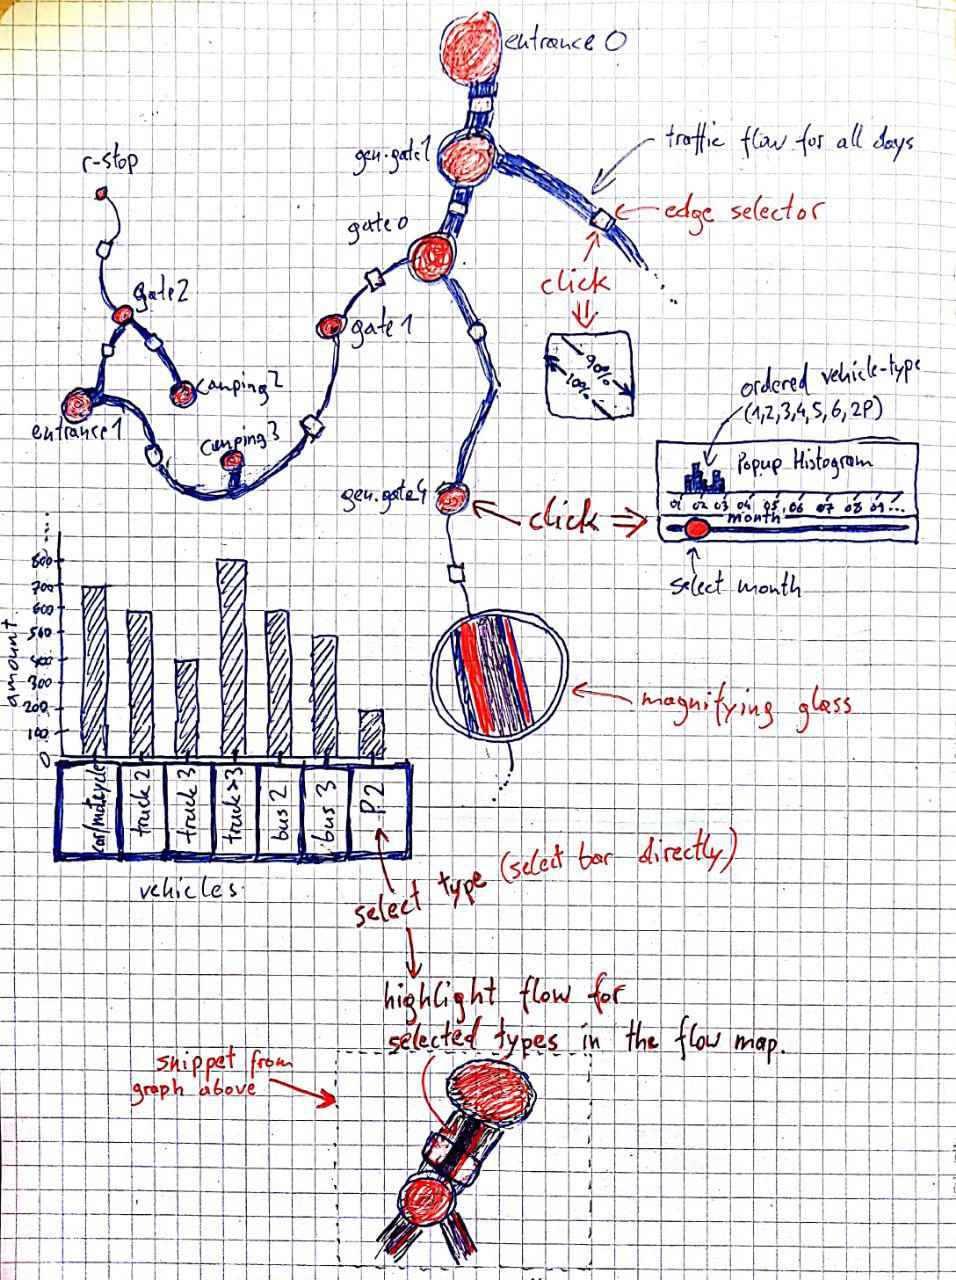
\includegraphics[scale=0.599]{Design2.jpg}	
	\caption{Design 2}
	\label{fig:design2}
\end{figure}

\paragraph*{Visualizing traffic flow.}
For my second design (\texttt{\hyperref[fig:design2]{Figure~\ref{fig:design2}}}) I wanted to show what roads are most frequently used overall, because this might correlate with the area where the birds decline the most.\\
One could argue, that the map from the rangers (as a visualization on its own) already contributes valuable information by revealing the camp- and road locations. Therefore, the map could be used to draw reasonable conclusions right away.
Since the map can be represented by a planar graph, I chose to visualize this with a \textit{flow map}. The sensors are represented by circle-shaped vertices. The vertices should have similar spacial placing like the sensor dots depicted on the ranger map. The paths of the vehicles are presented by merged edges which should also be approximated to the spatial layout of the ranger map. The edges grow in thickness according to the traffic intensity on the paths. The vertices also grow (in a continuous manner) in size to match the thickness of the edges (this is a questionable design choice and in hindsight, I should have drawn them with equal size).\\
The total amount of vehicles is presented in an additional barchart and lets \textit{Mitch} figure out what vehicle type is most common in the preserve.\\
Selecting a bar highlights the merged edges for the selected type and, while still visible, puts the unselected edges from the merged edge set in the background. This would then reveal the ratio between the selected type and the unselected types directly on the paths.\\
A drawback might be that the graph, in reality, is a directed graph, but is presented as undirected, leaving out valuable information in what directions the vehicles were going. Therefore, I implemented square-shaped edge selectors on the merged edges that, when clicked, will yield a popup. The popup then contains two parallel bi-directed arrows, with the same slope as the merged edges at the edge selector location, that present percentages of the directions that all the vehicles on that path were heading in.\\
Clicking on a vertex also yields a popup. This popup contains a timeline histogram with a slider to select the month. The histogram shows the total amount of vehicle types that were passing the sensor in the selected month. This might help \textit{Mitch} evaluate the traffic for a specific time domain on a specific path.\\
Additionally, a magnifying glass might also help revealing further traffic information, especially from thin edges. I prefer a magnifying glass over a fisheye lens, because the distortion obtained by a fisheye lens heavily impairs distance / length judgments and thus simply looks and feels horrible to me. I was playing with the idea, to show the histogram of a vertex when hovering the magnifying lens over said vertex. I figured the lens could eventually still be too small, also I wasn't brave enough to make a (much beloved) pie chart inside a magnified vertex. Therefore, the magnifying glass would show nothing new when dragged over a vertex.


\subsection*{Design 3}

\begin{figure}[h]
	\centering
	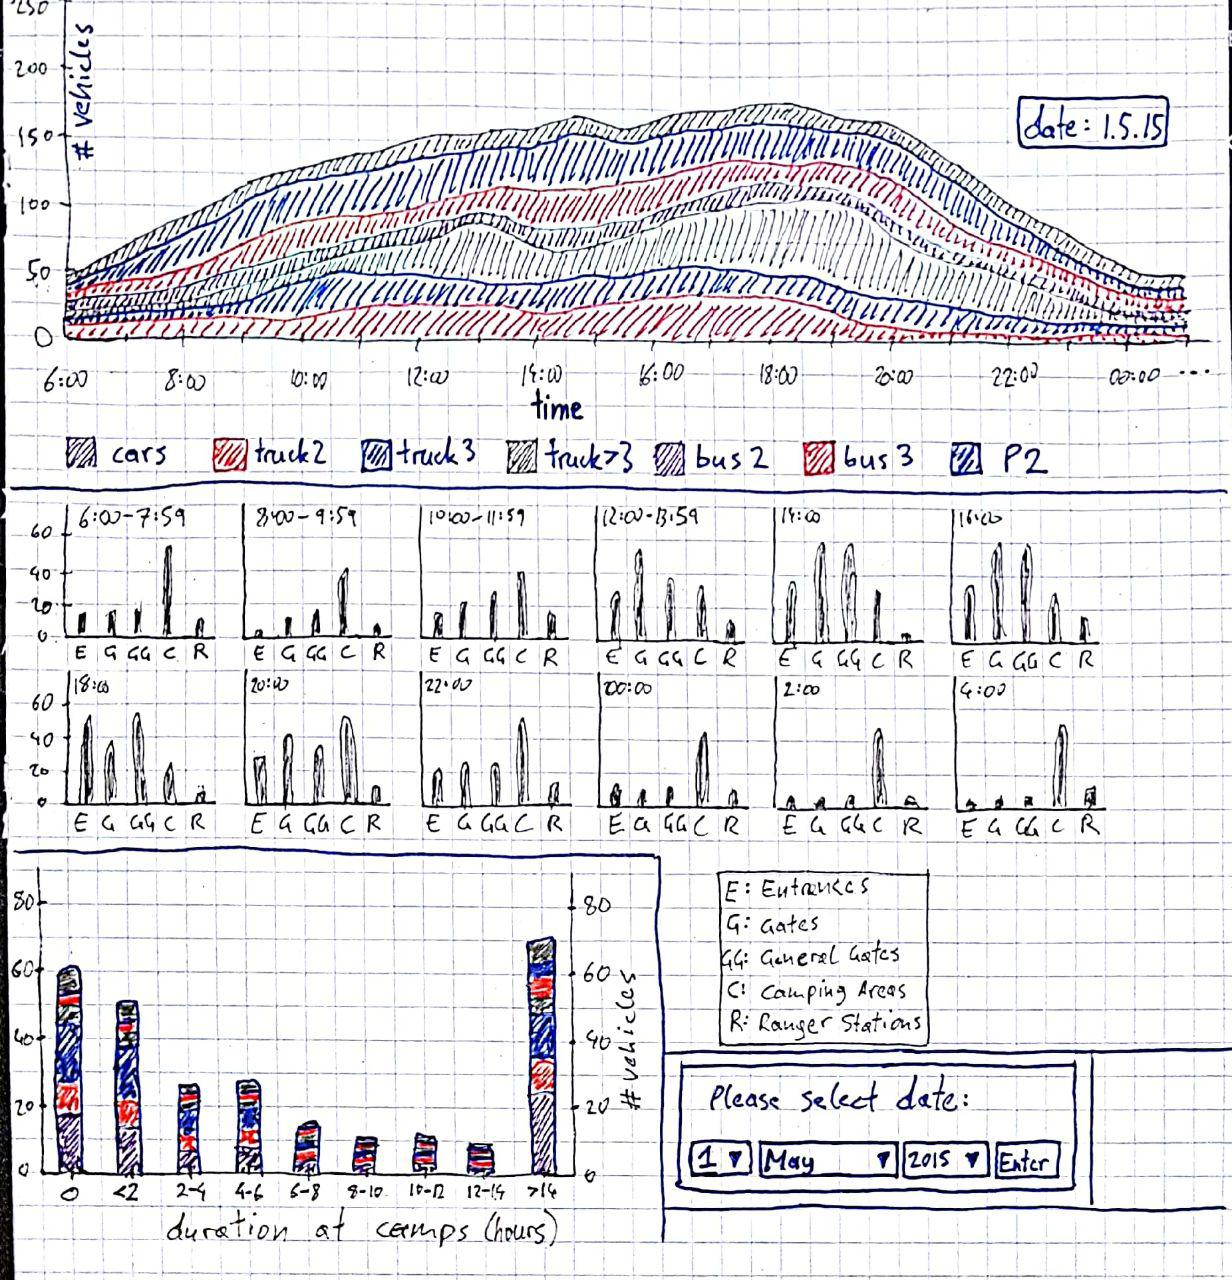
\includegraphics[scale=0.45]{Design3.jpg}	
	\caption{Design 3}
	\label{fig:design3}
\end{figure}

\paragraph{Visualizing traffic density (and traffic movement).}
For my last design (\texttt{\hyperref[fig:design3]{Figure~\ref{fig:design3}}}) I chose to work mainly with stacked visualization types to visualize traffic density. The stream graph shows the amount of vehicles that are in the preserve over one day. Since the amount of vehicles is \textit{quantitative} data, and the vehicles themselves are \textit{nominal} and few (i.e. \textit{colorable}) and time is an \textit{ordinal} attribute, this type of visualization was a perfect choice in my opinion\citep{munzner2015visualization}. The day can also be selected with the date selector in the bottom right corner of the design.\\
Below the stream graph I wanted to show movement between the different sensor types. Therefore, I drew histograms at different points in time that show the amount of vehicles currently present at each sensor type. This could have probably been animated as well, but I consider my approach to be superior over animation because the change in the five histogram bars would be too much to comprehend in an animation. Generally, in such cases, the amount of frames should always be reduced, i.e. convert from animation to side-by-side views. In total, there are twelve views distributed over two rows. It was of very importance to me that the views are row-aligned in order to be closer together. This should reduce cognitive load and there is only one line jump were \textit{Mitch} has to rely on his memory instead\citep{munzner2015visualization}. Everyone understanding the english language tends to read from left to right. This habit should also adapt to the side-by-side view.\\
Another thing that might interest \textit{Mitch} is the duration that vehicles spend at camping areas. Since the vehicle types are nominal and colorable,  the duration intervals are nominal and the amount of vehicles is quantitative, it made sense to create a stacked bar chart here\citep{munzner2015visualization}.


\section{Comparison}
I reckon \hyperref[fig:design2]{design 2} is probably a bit too complicated for \textit{Mitch}, also because it contains by far the most interaction from all three prototypes. Therefore, there is a high chance that he could overlook or miss some of it. That's why e.g. the \textit{edge selector} must be designed in a way, that \textit{Mitch} wants to click on it intuitively. I justified the \textit{vertex selector} earlier, stating that this might help \textit{Mitch} gain insight in the traffic over a month for a specific path. I felt the need to justify this because this gimmick somehow feels a bit tucked on. If I had to rethink my design, I would probably re-imagine the \textit{vertex selector} first.\\
However, I consider the \textit{flow map} itself extremely valuable, because it works good for visualizing the movements of objects from one location to another and it reduces visual clutter by merging all the edges. Therefore, it has high potential in conveying important information about the spacial traffic distribution.\\
I chose visualization types like \textit{flow maps}, \textit{bar charts} and \textit{histograms} that work for large amounts of data. (Also this is so trivial I can't believe I'm even writing this, but the bar chart works for nominal data (like \textit{vehicle type}) and line charts for ordinal (like \textit{time}), therefore the \textit{bar chart}.)\\

I consider \hyperref[fig:design1]{design 1} to be the most developed one because the data is transformed into something else and then visualized by a \textit{SPLOM} and \textit{PC}. I chose the time range to be one day because this should reduce the amount of scatterpoints to a few hundred. This kind of time filtering is needed in order to visualize the data properly. Too many points would probably yield in a \textit{PC}-hairball, revealing almost no information at all. A drawback might be that the \textit{SPLOM} might not show any correlation at all, and then I would have to tackle the problem differently.\\
It is hard to compare this design to the previous one, because the tasks differ. Also one is an overview and the other one provides detailed visualization.\\

The  \hyperref[fig:design3]{third design} kind of merges the two previous tasks. It looks mainly at traffic density (behavior) via the \textit{stream graph}, \textit{stacked bar chart} and \textit{gate histograms} and a little bit at traffic flow by examining the gates at different steps in time via the side-by-side view of the \textit{gate histograms}. This design would also work as an overview, since all visualization types are capable to display large amounts of data.

\section{Summary}
In order to create my visualizations I needed estimates about the amount of data entries with respect to different attribute constraints. Luckily, the data was already there and I could lookup different things by pre-filtering in \textit{Excel}. This helped in choosing time ranges for the detail design views.\\

I noticed that only arrivals at gates / camps are tracked, but no departures. Therefore, we could come up with the assumption, that campers could also camp somewhere along the way before the next gate. However, in the Lekagul Preserve description file, it clearly states, that camping and cycling are only allowed in designated areas. So if the rangers do their job properly, (which we could check by visualization) it is reasonable to strongly assume the opposite.\\

Also, there is no information about the birds themselves. This fact limited the visualization space by narrowing the visualization tasks to the traffic only.\\

The third design addresses both tasks (traffic flow and traffic behavior) and would also work not only for a single day, but also as an overview, since all visualization types are capable to display large amounts of data as well. Having this kind of flexibility and a high chance of displaying valuable information (compared to the first design) I consider this to be my best prototype overall.

\subsection{Realization in Tableau}
I imagine the \textit{flow map} would be the hardest to do in \textit{Tableau}, because it would have to be drawn by hand as far as I know\citep{munzner2015visualization}. Also one would have to calculate the edges and implement all the interactivity, which is a bit of an overkill, I think.  The first design would require the data to be transformed into a duration table fist, which is manageable, but Tableau doesn't support \textit{PC} at the moment, which is unfortunate. The easiest design to realize would probably be the third prototype. Tableau can easily handle stream graphs, histograms and stacked barplots.

\bibliographystyle{plainnat}
\bibliography{a01403753_A4}

\end{document}